%%=============================================================================
%% Resultaten
%%=============================================================================

\chapter{Resultaten}%
\label{ch:resultaten}

\section{\IfLanguageName{dutch}{Brute Force Attack op WordPress Omgevingen met Beveiligingsplugins}{Brute Force Attack on WordPress enviroment with securityplugins}}
Binnen de context van webbeveiliging zijn brute force aanvallen een veelvoorkomende methode waarbij aanvallers trachten toegang te krijgen tot een systeem 
door herhaaldelijk logins of wachtwoorden te raden. Dit type aanval kan bijzonder schadelijk zijn voor systemen zoals WordPress, die veel 
gebruikt worden voor het bouwen van websites.In dit hoofdstuk onderzoeken we de effectiviteit van verschillende penetratietesttools bij het uitvoeren van 
brute force aanvallen op een WordPress-omgeving beveiligd met de Wordfence plugin. Het doel is niet om de beveiligingsplugins zelf te testen, maar om de 
prestaties, de mogelijkheden en bruikbaarheid van de tools Burp Suite, Metasploit en OWASP ZAP met elkaar te vergelijken. Deze analyse zal helpen vaststellen welke tool 
het meest effectief en gebruiksvriendelijkst is voor het tonen van kwetsbaarheden in een beschermde WordPress-omgeving.

\subsection{\IfLanguageName{dutch}{Resultaat met burp suite}{result with burp suite}}
\begin{figure}
    \centering
    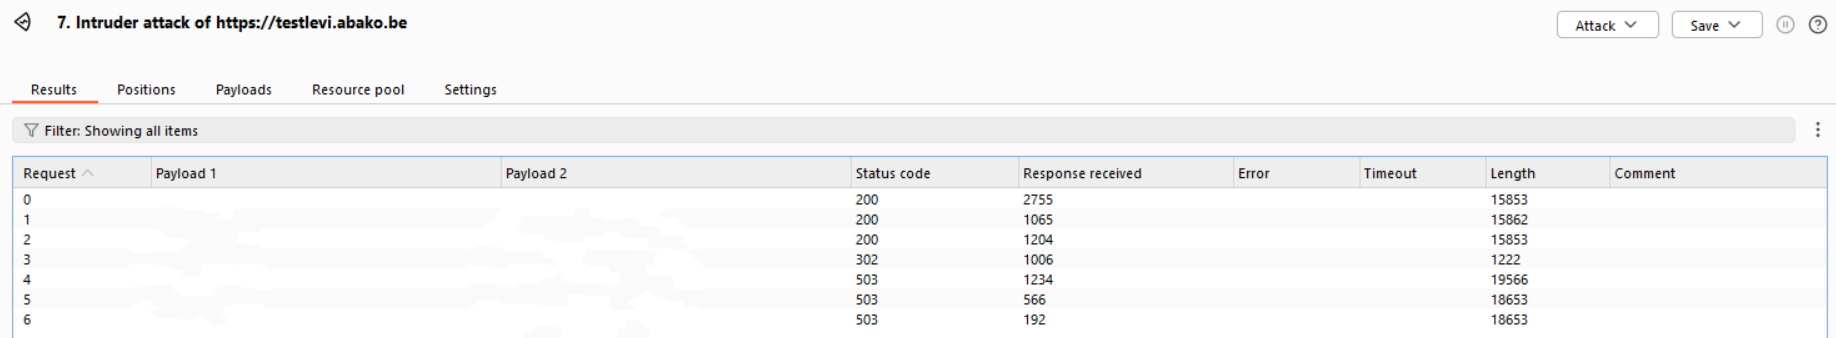
\includegraphics[height=0.1\textheight]{burp-suite_bruteforce_wordpressplugins_blurred.png}
    \caption[Burp suite brute force attack op wordpress applicatie met beveiligingsplugin]{Burp suite brute force attack op wordpress applicatie met beveiligingsplugin}
\end{figure}
De brute force attack op een WordPress omgeving met wordfence beveiligingsplugin werd uitgevoerd met behulp van Burp Suite Community Edition. Tijdens de test viel het 
op dat enkele functionaliteiten beperkt waren vanwege de beperkingen van de Community Edition. Dit beperkte de mogelijkheden van het uitvoeren van een volledige 
pentest, maar het voordeel van Burp Suite is dat er veel documentatie en tutorials beschikbaar zijn op het internet, wat nuttig kan zijn bij het oplossen van 
eventuele problemen tijdens het gebruik van de tool.

Naast de brute force attack werd er ook een SQL-injectie pentest uitgevoerd met Burp Suite. In de WordPress-omgeving met beveiligingsplugins werd de SQL-injectie aanval 
effectief gedetecteerd en geblokkeerd door de beveiligingsmaatregelen van Wordfence. Dit toont aan dat de plugins niet alleen bescherming bieden tegen brute force 
aanvallen, maar ook tegen SQL-injecties, wat cruciaal is voor de algehele beveiliging van de applicatie

\subsection{\IfLanguageName{dutch}{Resultaat met metasploit}{result with metasploit}}
\begin{figure}
    \centering
    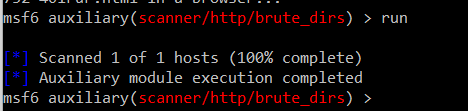
\includegraphics[height=0.1\textheight]{metasploit_brute_wordpressplugin.png}
    \caption[Metasploit brute force attack op wordpress applicatie met beveiligingsplugin]{Metasploit brute force attack op wordpress applicatie met beveiligingsplugin}
\end{figure}
Metasploit is een populair open-source framework voor beveiligingstests, dat vooral wordt ingezet voor het ontwikkelen en implementeren van exploit-codes. 
Met dit framework kunnen systemen worden beoordeeld op veiligheid door actief kwetsbaarheden te exploiteren en te identificeren. 
Metasploit beschikt over honderden exploit-modules die een breed scala aan bekende kwetsbaarheden dekken, waardoor het als een belangrijk 
instrument kan worden gezien in de toolkit van veel cybersecurity-professionals.

In een praktische toepassing werd Metasploit gebruikt om een brute force attack uit te voeren op een WordPress-omgeving die beveiligd was met de Wordfence plugin. 
Voor deze test diende de tool via de terminal bediend worden. Hoewel dit als een beperking kan worden gezien, biedt Metasploit een uitgebreid scala aan 
mogelijkheden voor het uitvoeren van penetratietests. De tool stelt gebruikers in staat om diverse aanvalsscenario's te simuleren en levert een uitgebreide reeks 
modules voor het uitvoeren van verschillende soorten beveiligingstests. Deze flexibiliteit en diepgang maken van Metasploit een waardevolle keuze voor professionals die 
uitgebreide beveiligingstests willen uitvoeren op complexe netwerken en systemen.

\subsection{\IfLanguageName{dutch}{Resultaat met OWASP ZAP}{result with OWASP ZAP}}
\begin{figure}
    \centering
    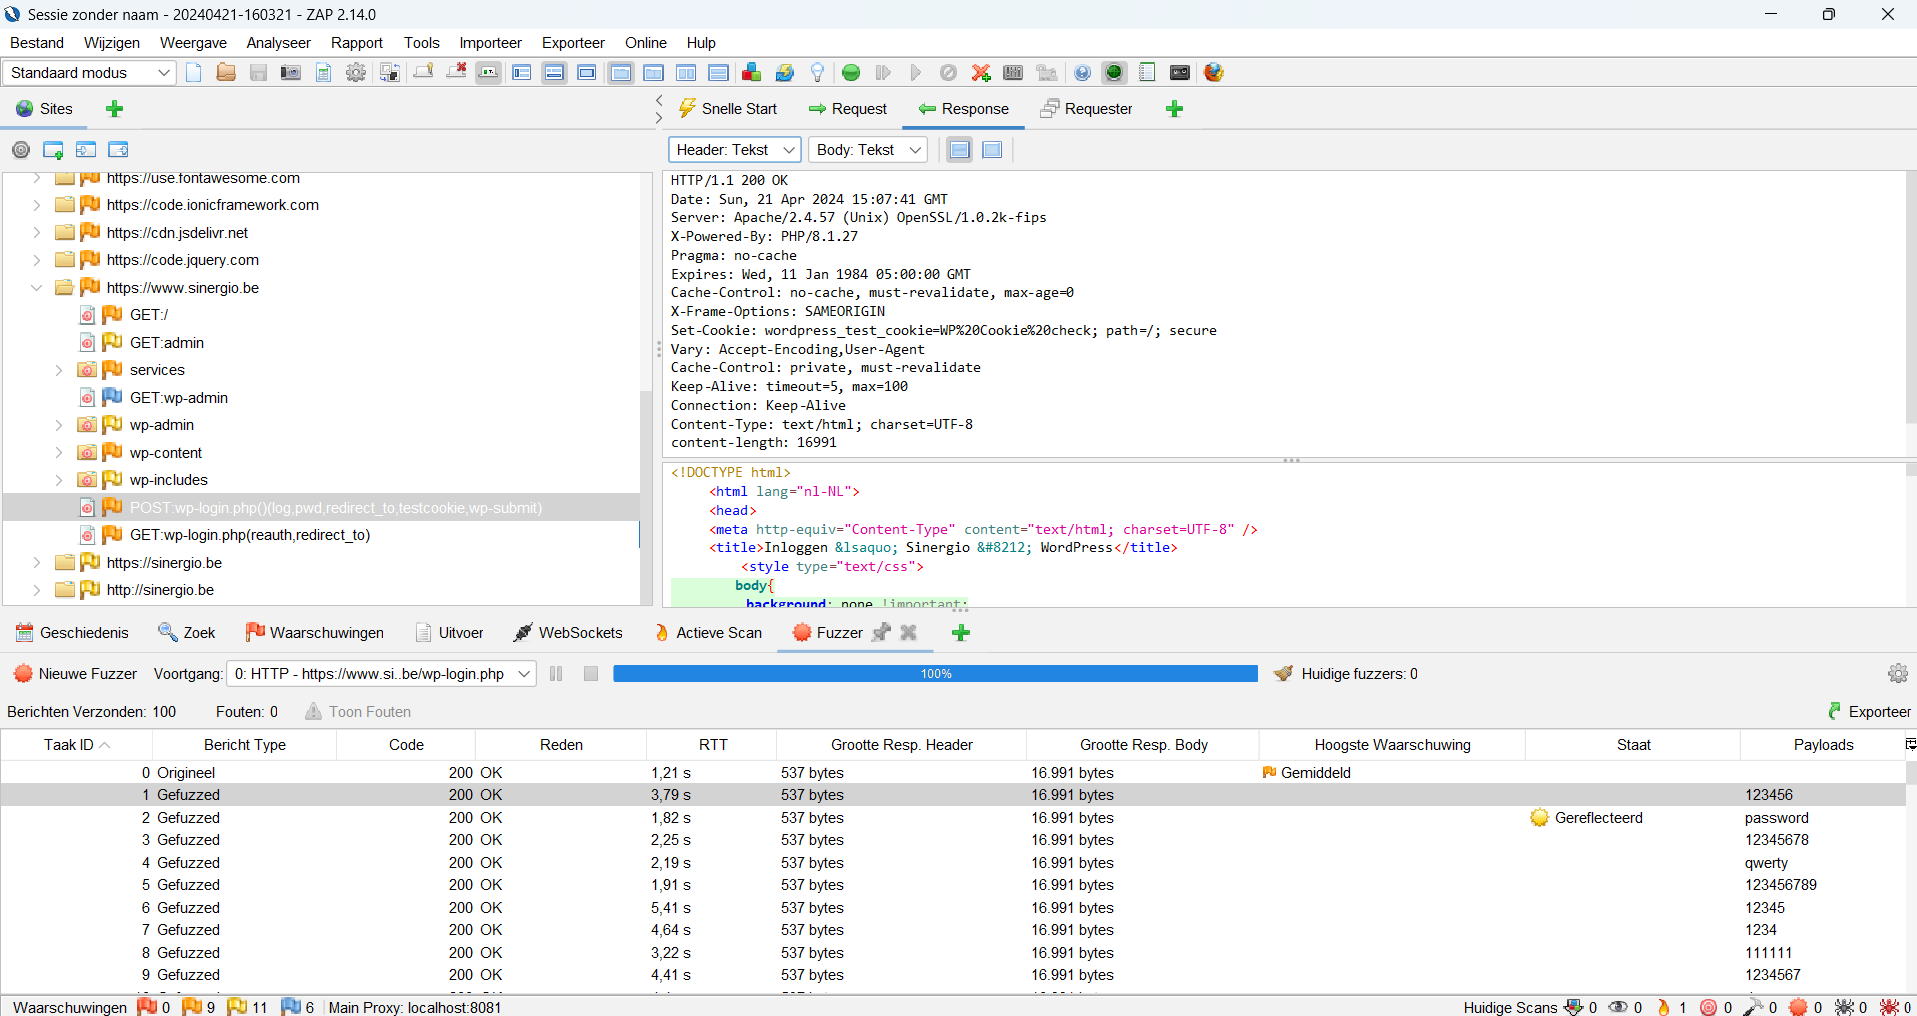
\includegraphics[height=0.3\textheight]{ZAP_brute_wordpressplugin.png}
    \caption[OWASP ZAP brute force attack op wordpress applicatie met beveiligingsplugin]{OWASP ZAP brute force attack op wordpress applicatie met beveiligingsplugin}
\end{figure}

Voor de brute force attack op de WordPress omgeving met wordfence werd OWASP ZAP gebruikt, een open source tool die bekend staat om zijn gebruiksgemak. 
Wat opviel bij het gebruik van OWASP ZAP was dat de resultaten van de testen vergelijkbaar waren als bij de betalende Burp Suite, maar dan met een open source alternatief. 
Dit maakt van OWASP ZAP een aantrekkelijke keuze voor organisaties die op zoek zijn naar een kosteneffectieve oplossing voor het uitvoeren van beveiligingstests.

Daarnaast werd met OWASP ZAP ook een SQL-injectie pentest uitgevoerd. De beveiligingsplugin van WordPress detecteerde en blokkeerde de SQL-injectie aanval effectief, 
wat wederom de betrouwbaarheid van de beveiligingsmaatregelen aantoont. OWASP ZAP's intuïtieve interface en effectieve testresultaten maken het een sterke concurrent 
voor andere penetratietesttools. Een voorbeeld van deze pentest kan hier worden teruggevonden \ref{fig:sql-injection}.

\section{\IfLanguageName{dutch}{Vergelijking van omgevingen}{Comparison of environments}}
%\begin{figure}
%    \centering
%    \includegraphics[height=0.1\textheight]{ }
%    \caption[Brute force aanval op een wordpress applicatie zonder beveiligingsplugins (foto moet nog geblurred worden)]{Brute force aanval op een wordpress site zonder beveiligingsplugins}
%\end{figure}
\subsection{\IfLanguageName{dutch}{WordPress Zonder Beveiligingsplugins}{WordPress without securityplugins}}
De eerste testomgeving was een standaard WordPress-applicatie zonder enige vorm van beveiligingsplugins. De resultaten toonden aan dat deze 
omgeving bijzonder kwetsbaar was voor brute force aanvallen. Aanvallers zijn in staat om binnen enkele minuten toegang te verkrijgen door middel 
van standaard gebruikersnamen zoals 'admin' en algemeen bekende zwakke wachtwoorden. Deze bevindingen benadrukken de noodzaak voor 
basisbeveiligingsmaatregelen, zoals het instellen van sterke wachtwoorden en het gebruik van moeilijkere gebruikersnamen om de initiële 
beveiliging te verstevigen.

\begin{figure}
    \centering
    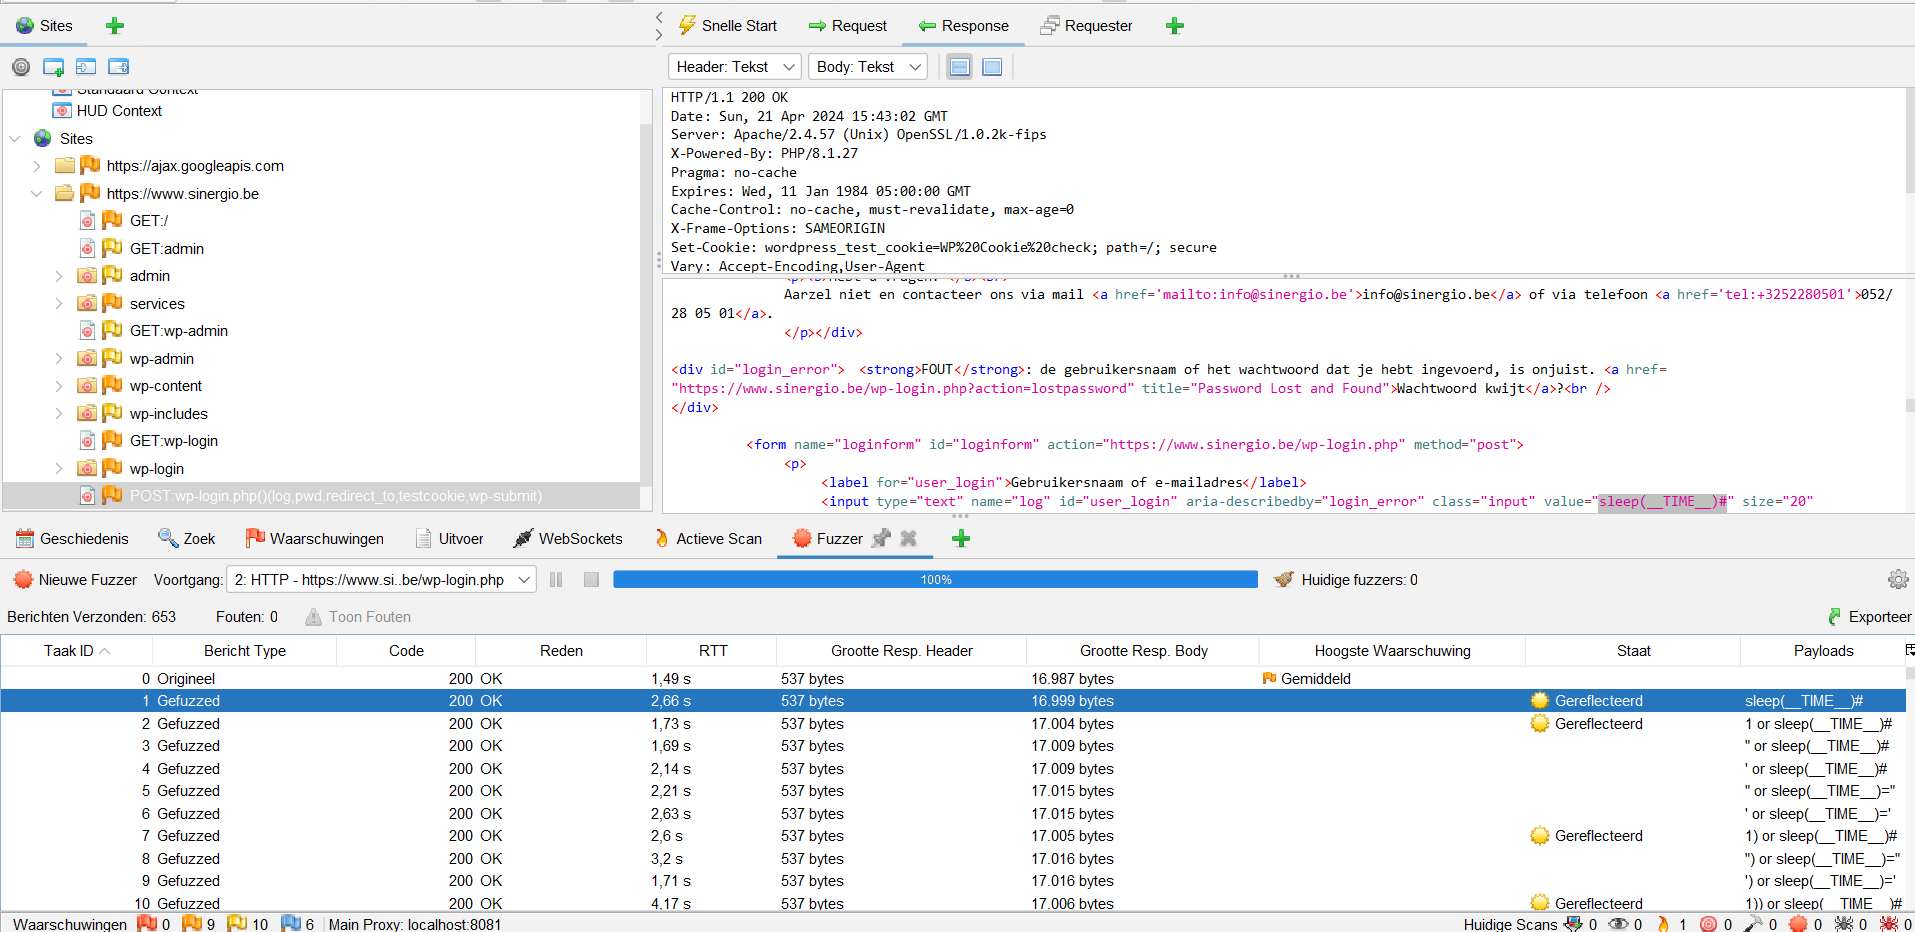
\includegraphics[height=0.2\textheight]{zap_sql-injection_wordpressplugin.png}
    \caption[SQL-injection aanval op een wordpress applicatie met beveiligingsplugins]{SQL-injection aanval op een wordpress applicatie met beveiligingsplugins}
    \label{fig:sql-injection}
\end{figure}
\subsection{\IfLanguageName{dutch}{WordPress Met Beveiligingsplugins}{WordPress with securityplugins}}
De tweede test-omgeving, een WordPress-installatie uitgerust met specifieke beveiligingsplugins zoals Wordfence, liet een aanzienlijke 
verbetering zien in beveiliging tegen brute force-aanvallen. De plugins die werden getest, bieden functionaliteiten zoals limieten 
op inlogpogingen, directe accountvergrendeling bij verdachte activiteiten en real-time monitoring en alerts. Deze maatregelen 
leiden tot een snelle detectie en blokkering van aanvalspogingen, waardoor de veiligheid van de omgeving aanzienlijk werd verhoogd.

\begin{figure}
    \centering
    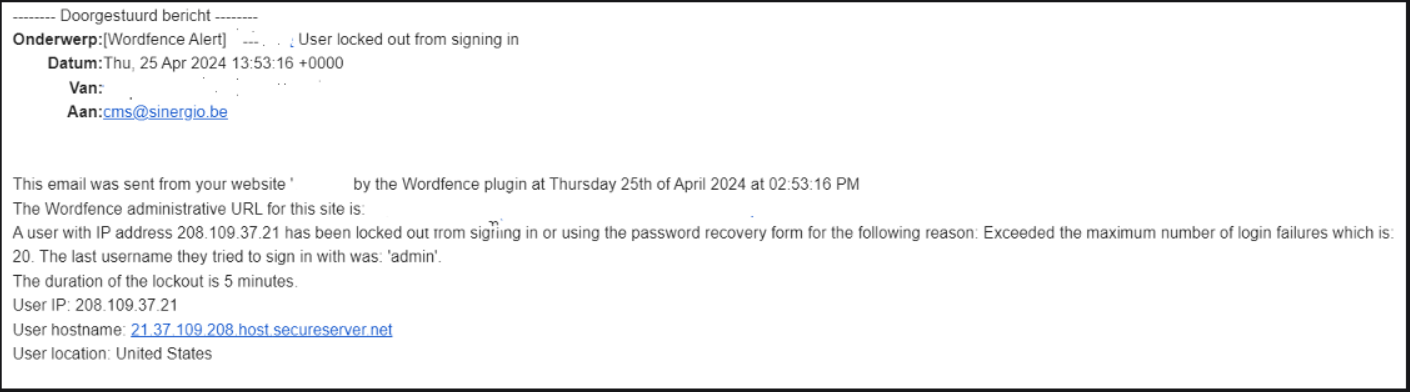
\includegraphics[height=0.2\textheight]{foute_login_mail_blurred.png}
    \caption[E-mail over geblokkeerde inlog poging]{E-mail over geblokkeerde inlog poging}
    \label{fig:geblokkeerde-login}
\end{figure}
Wanneer een gebruiker bijvoorbeeld het maximum aantal mislukte inlogpogingen overschrijdt, stuurt Wordfence een alert. 
Een typische melding kan er als volgt uitzien: "A user with IP address 208.109.37.21 has been locked out from signing in or 
using the password recovery form for the following reason: Exceeded the maximum number of login failures which is: 20. The 
last username they tried to sign in with was: 'admin'. The duration of the lockout is 5 minutes."

Deze melding bevat belangrijke informatie zoals:
\begin{itemize}
    \item IP-adres van de aanvaller: In dit geval 208.109.37.21.
    \item Hostname: 21.37.109.208.host.secureserver.net.
    \item Locatie van de gebruiker: United States.
    \item Gebruikersnaam: De laatste gebruikersnaam waarmee geprobeerd werd in te loggen, bijvoorbeeld 'admin'.
    \item Reden voor blokkering: Het overschrijden van het maximum aantal mislukte inlogpogingen, hier vastgesteld op 20.
    \item Duur van de blokkering: In dit geval 5 minuten.
\end{itemize}
Als deze limiet is bereikt, ontvang je een vergelijkbare alert met details over de geblokkeerde gebruiker en de 
blokkeringstijd.

Verder biedt Wordfence ook directe accountvergrendeling bij verdachte activiteiten. Dit blokkeert onmiddellijk een 
account wanneer bijvoorbeeld een plotseling groot aantal mislukte inlogpogingen wordt gedetecteerd. De alert geeft 
aan welk account is vergrendeld en de reden voor de vergrendeling.

Wordfence biedt daarnaast real-time monitoring van je website, waarbij verdachte activiteiten direct worden gemeld. 
Deze alerts kunnen variëren van verdachte inlogpogingen tot pogingen om kwetsbaarheden in plugins of thema's te misbruiken.
Een voorbeeld van een dergelijke alert kan je hier zien \ref{fig:geblokkeerde-login}. 

Deze resultaten onderstrepen het belang van het toepassen van gespecialiseerde beveiligingsuitbreidingen in populaire 
CMS-systemen, wat aantoont dat zelfs fundamentele beveiligingsplugins een significante bescherming kunnen bieden.
\begin{figure}
    \centering
    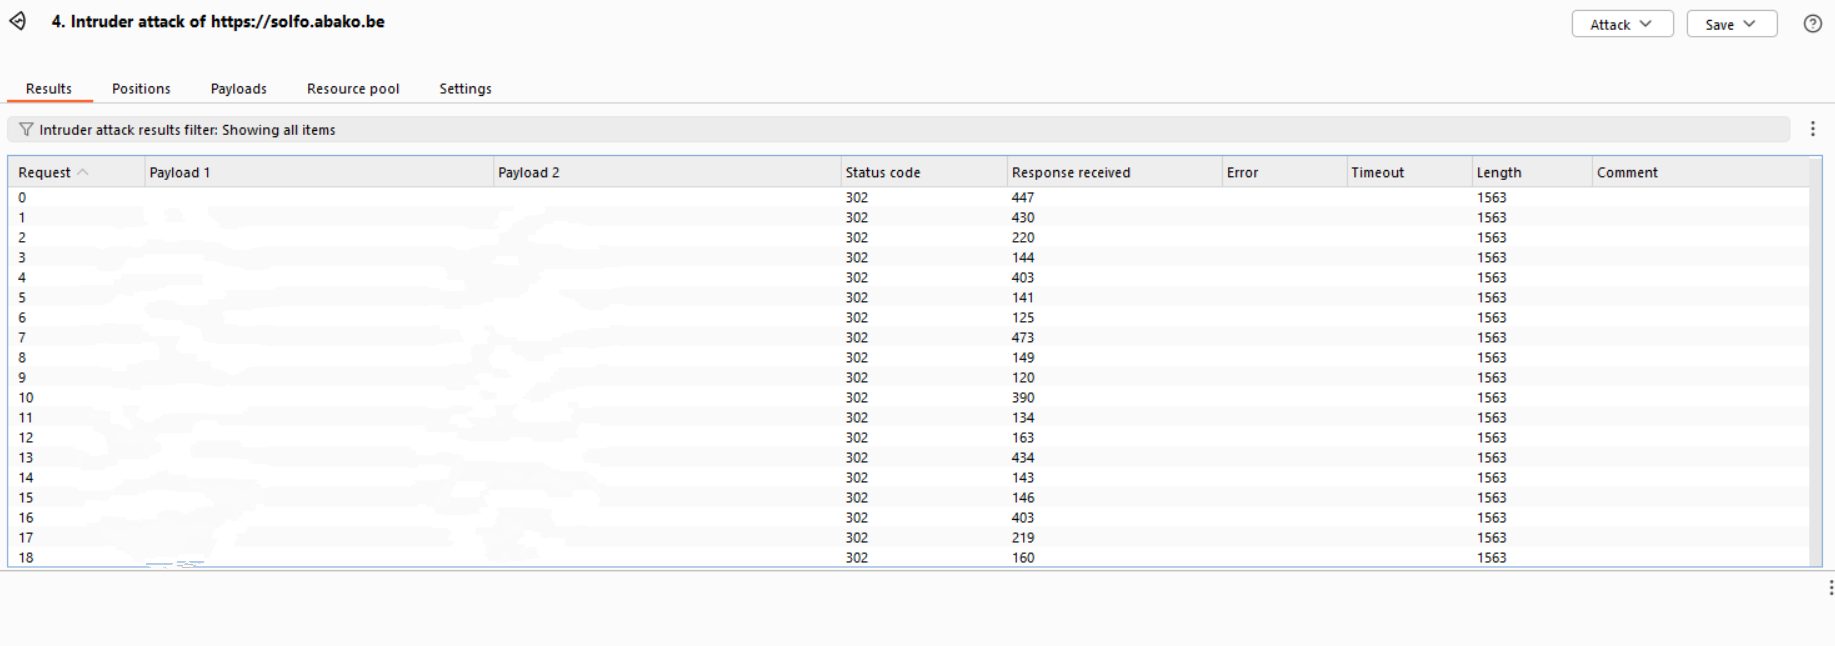
\includegraphics[height=0.2\textheight]{burp-suite_bruteforce_laravel_blurred.png}
    \caption[Brute force aanval op een laravel applicatie]{Brute force aanval op een laravel applicatie}
    \label{fig:laravel-brute-force}
\end{figure}
\subsection{\IfLanguageName{dutch}{Laravel Applicatie}{Laravel Application}}
Na de aanval analyseerden we de resultaten. Er werden geen succesvolle inlogpogingen gedetecteerd zoals je kan zien op foto \ref{fig:laravel-brute-force}, wat erop wijst dat de 
gebruikersnamen en wachtwoorden sterk genoeg waren om brute force aanvallen te weerstaan. Bovendien reageerde het systeem 
effectief op de aanvalspogingen door IP-adressen te blokkeren en CAPTCHA's te tonen. Een CAPTCHA is zijn een reactietest 
die in de gegevensverwerking wordt gebruikt om te bepalen of er al dan niet sprake is van een menselijke gebruiker. Dit toont aan dat er goede 
beveiligingsmaatregelen zoals account lockout policies en rate limiting waren geïmplementeerd.

In ons gedetailleerde rapport beschreven we de methodologie, de gebruikte tools, de configuraties, en de uitkomsten van de 
test. Hoewel de brute force aanval niet succesvol was, benadrukten we het belang van continue beveiligingsmonitoring en 
periodieke tests om de beveiliging up-to-date te houden. We gaven aanbevelingen zoals het blijven versterken van het 
wachtwoordbeleid, het implementeren van multi-factor authenticatie (MFA) voor extra beveiligingslagen, en het gebruik 
van intrusion detection en prevention systems (IDPS) om ongeautoriseerde toegangspogingen vroegtijdig te detecteren en 
te stoppen.